\documentclass[11pt,a4paper]{article}
\usepackage[utf8]{inputenc}
\usepackage[margin=1in]{geometry}
\usepackage{amsmath,amssymb,amsfonts}
\usepackage{graphicx}
\usepackage{booktabs}
\usepackage{hyperref}
\usepackage{cite}
\usepackage{microtype}

\hypersetup{
    colorlinks=true,
    linkcolor=blue,
    citecolor=blue,
    urlcolor=blue
}

\title{\textbf{Is Social Bias Concentrated and Localizable in Sparse Mixture-of-Experts?\\A Post-Hoc Game-Theoretic Analysis}}
\author{\textbf{Georgia Institute of Technology} \\ \texttt{\{author\}@gatech.edu}}
\date{July 2026}

\begin{document}

\maketitle

\begin{abstract}
Recent scaling of Large Language Models (LLMs) has been dominated by sparse Mixture-of-Experts (MoE) architectures, which partition network capacity into routed, modular experts. This structural modularity has spurred an influential ``localizability'' narrative: that network behaviors, factual associations, and biases are cleanly isolated within specialized, monosemantic experts, offering an elegant substrate for targeted editing and steering. In this paper, we conduct the first comprehensive post-hoc, game-theoretic bias-attribution study on open MoE models to empirically evaluate this claim. Specifically, we investigate four fundamental research questions: (1) Does bias attribution become more concentrated as routing sparsity increases? (2) Is bias more localizable in MoEs than in matched dense counterparts? (3) Is expert-level bias a property of individual modular units or collective coalitions? and (4) Is bias specialized to specific demographic subgroups?

Using a novel \textbf{routing-contrast Shapley value formulation} across StereoSet, BBQ, and WinoGender, we audit a diverse sparsity ladder of six open MoE models (spanning routing sparsity ratios $N_A/N$ from $0.016$ to $0.250$, where $N_A/N$ is the active expert ratio representing the number of active routed experts per token, $N_A$, divided by the total number of experts in that MoE layer, $N$) and compare them directly to matched dense baselines. Decisively challenging the modularity-fairness myth, we find that: (i) routing sparsity does not scale with bias concentration, as all audited MoEs exhibit near-maximum attribution entropy ($H \approx 0.88 - 0.92$, where a normalized Shannon entropy $H=1.0$ indicates perfect uniform diffusion and $H=0.0$ indicates absolute single-expert concentration); (ii) matched dense models actually exhibit \textit{more} concentrated bias profiles; (iii) early-layer bias is dominated by complex, non-additive pairwise synergies ($>70\%$); and (iv) although diffuse, biases are demographically specific, triggering distinct subsets of experts across demographic cohorts. Our causal ablation experiments validate these game-theoretic findings, indicating that social bias is a systemic, diffuse property of sparse MoEs, and that single-expert debiasing techniques are fundamentally misguided.
\end{abstract}

\section{Introduction}
The transition from dense autoregressive transformers to sparse Mixture-of-Experts (MoE) architectures represents a pivotal paradigm shift in foundation model engineering. Sparse routing decouples total parameter capacity from training and inference floating-point operations (FLOPs), enabling state-of-the-art architectures such as GPT-4, DeepSeek-V3, Qwen3, OLMoE, GPT-OSS, and DBRX to achieve remarkable performance.

Concurrently, a fast-growing interpretability literature has emerged, championing the ``modular monosemanticity'' of sparse MoEs. This perspective argues that because experts are routed sparsely, they naturally specialize in specific syntactic, semantic, or conceptual domains (e.g., \textit{The Expert Strikes Back} \cite{expert_strikes_back}; \textit{Sparsity \& Superposition in MoE} \cite{sparsity_superposition_moe}). A direct, unexamined corollary of this modularity narrative is the \textbf{localizability thesis}: \textit{social and demographic stereotyping biases are localized in a small, identifiable ``committee'' of experts, which can be easily targeted for surgical debiasing or parameter steering.}

If the localizability thesis holds, it introduces an elegant, computationally efficient mechanism for LLM alignment: auditors can locate the handful of ``biased experts'' in a deployed model and ablate or adjust them without expensive full-parameter retraining. If the thesis is false, however, it corrects the prevalent ``modularity-interpretabilty'' narrative with a crucial safety and fairness caveat, showing that modular routing does not prevent systemic, diffuse social stereotyping.

In this study, we formalize and empirically evaluate the localizability of social stereotype bias in sparse MoEs. We treat the active experts at each layer as players in a cooperative game and employ a game-theoretically grounded \textbf{routing-contrast Shapley value} to attribute the model's output bias payoff. We construct a comprehensive ``sparsity ladder'' comprising six open MoE architectures spanning a massive range of routing sparsity $N_A/N$ (defined as the active expert fraction, representing the ratio of active routed experts $N_A$ per token to total available experts $N$ per layer):
\begin{itemize}
    \item \textbf{OLMoE-1B-7B} ($N_A/N \approx 0.016$);
    \item \textbf{GPT-OSS-120B} ($N_A/N \approx 0.031$);
    \item \textbf{Gemma 4 26B} ($N_A/N \approx 0.063$);
    \item \textbf{Phi-3.5-MoE} ($N_A/N \approx 0.125$);
    \item \textbf{Mixtral-8x7B} ($N_A/N \approx 0.250$); and
    \item \textbf{DBRX-instruct} ($N_A/N \approx 0.250$).
\end{itemize}
We evaluate these alongside three dense models that serve as baseline controls:
\begin{itemize}
    \item \textbf{OLMo-7B} ($N = 32$ layers);
    \item \textbf{Phi-3.5-mini} ($N = 32$ layers); and
    \item \textbf{Llama-3.1-8B} ($N = 32$ layers).
\end{itemize}

\subsection{Core Research Questions and Results-at-a-Glance}
To systematically analyze how social stereotype bias is organized inside MoE networks, we outline and address four central research questions:

\begin{enumerate}
    \item \textbf{RQ1 (Sparsity Scaling \& Concentration):} Across MoE models of increasing routing sparsity (lower active expert fraction $N_A/N$), does bias attribution become more concentrated in fewer experts? I.e., does sparsity $\rightarrow$ concentration?
    \begin{itemize}
        \item \textit{Verdict:} \textbf{Rejected (H1 Rejected).} We find no monotonic relation between routing sparsity and bias concentration. For instance, GPT-OSS-120B ($N_A/N = 0.031$, $H = 0.880$, Gini = $0.724$, where Gini is the inequality coefficient measuring attribution concentration across experts, ranging from $0.0$ for perfect equality to $1.0$ for maximum concentration) is more concentrated than OLMoE-1B-7B ($N_A/N = 0.016$, $H = 0.900$, Gini = $0.599$) despite OLMoE being twice as sparse. Scale, training objectives, and data alignment override the routing sparsity ratio.
    \end{itemize}
    
    \item \textbf{RQ2 (MoE vs. Dense Localizability):} At matched training capability and family, is bias more localizable (lower entropy of attribution) in MoE models than in their dense counterparts?
    \begin{itemize}
        \item \textit{Verdict:} \textbf{Rejected (H2 Rejected).} Matched dense baselines (e.g., OLMo-7B, Phi-3.5-mini) actually exhibit significantly \textit{more} concentrated bias profiles ($H \approx 0.63 - 0.76$) than MoEs ($H \approx 0.88 - 0.92$), though this comparison is subject to a multi-scale granularity confound (layer-level vs. expert-level players).
    \end{itemize}
    
    \item \textbf{RQ2b (Collectivity / Synergy):} Is expert-level bias a property of individual modular units, or does it emerge from collective, non-linear expert coalitions (synergy, representing cooperative, non-additive expert-interaction effects)?
    \begin{itemize}
        \item \textit{Verdict:} \textbf{Synergy Dominates.} In early layers, $70.2\% - 74.4\%$ of total attribution is driven by non-additive pairwise synergy. This demonstrates that experts act as ``standing committees'' rather than isolated biased agents, and individual expert-contrast metrics underestimate the true diffuseness of bias.
    \end{itemize}
    
    \item \textbf{RQ3 (Demographic Specificity):} Across distinct demographic cohorts, do different experts fire, or does the same set of experts flip their bias contributions?
    \begin{itemize}
        \item \textit{Verdict:} \textbf{Subgroup-Specific Subnetworks.} Social bias is subgroup-specific at the expert level. We observe non-trivial Jensen-Shannon divergence ($D_{JS}$, a symmetric distance metric between probability distributions, where $D_{JS}=0.0$ indicates identical expert activation profiles and $D_{JS}=1.0$ indicates completely disjoint subsets of active experts) between absolute attribution distributions across cohorts (e.g., gender-focused vs. race-focused prompts). While bias is diffuse within each cohort, distinct, non-overlapping subsets of experts are activated based on specific demographic targets.
    \end{itemize}
\end{enumerate}

\subsection{Central Hypotheses and Verdicts}
Specifically, we test three central hypotheses spanning the sparsity-to-density axis:
\begin{itemize}
    \item \textbf{$H_1$ (Sparsity-to-Concentration):} Bias-Shapley concentration is monotonically increasing as routing sparsity ($N_A/N$) decreases. Sparser models (lower $N_A/N$) will exhibit lower normalized Shannon entropy ($H$) of bias attribution. \textbf{[Verdict: REJECTED]}
    \item \textbf{$H_2$ (MoE-vs-Dense Localizability):} At matched training data and computational capability, an MoE model exhibits a significantly more localized (concentrated) bias profile than its dense sibling ($H_{\text{MoE}} < H_{\text{dense}}$). \textbf{[Verdict: REJECTED]}
    \item \textbf{$H_0$ (Diffuse Bias Null):} Bias attribution is near-maximally diffuse and stable across all MoE models ($H \approx 0.88 - 0.92$), correcting modular localizability assumptions. \textbf{[Verdict: STRONGLY SUPPORTED]}
\end{itemize}

\subsection{Key Contributions}
\begin{itemize}
    \item \textbf{Systematic MoE Bias Audit:} We conduct the first post-hoc game-theoretic bias-attribution study on MoE LLMs, correcting the prevalent ``modularity-interpretabilty'' narrative with a crucial safety and fairness caveat.
    \item \textbf{Tractable Exact Shapley Value:} We leverage top-$K$ sparsity to compute near-exact active-coalition expert-Shapley values, demonstrating an MoE-specific interpretability capability that is impossible in dense models.
    \item \textbf{Empirical Reject of Localizability:} We build a rigorous ``sparsity ladder'' comprising six open MoE models and matched dense controls to map the entire sparsity-to-density axis, proving that social bias is a diffuse, systemic property of MoEs.
    \item \textbf{Causal Ablation \& Interaction Analysis:} We quantify early-layer synergy fractions ($>70\%$) and perform physical zero-ablation sweeps to causally validate our game-theoretic findings, proving that single-expert debiasing is fundamentally misguided.
\end{itemize}

\section{Related Work}
\subsection{Mechanistic Interpretability and Attribution in LLMs}
Mechanistic interpretability seeks to map high-level behaviors in neural networks to discrete circuits and components \cite{dissecting_bias}. Techniques such as activation patching and Edge-Attribution Patching (EAP) have successfully mapped factual association circuits in dense transformers. However, scaling these causal interventions to networks with tens of billions of parameters is exceptionally expensive. 

\subsection{Game-Theoretic Attribution (Shapley Values)}
To assign principled contributions to individual components, researchers have turned to cooperative game theory. The Shapley value provides a unique, axiomatically justified allocation of payoffs among a set of players \cite{realexp}. While full-scale Shapley computation over dense layers is computationally intractable (requiring $2^D$ model evaluations where $D$ is the hidden dimension), sparse MoEs present a unique structural advantage. 

Specifically, \textbf{Shapley-MoE} \cite{shapley_moe} established the core methodological precedent for expert-level Shapley evaluation, showing that sparse top-$K$ routing makes exact active-coalition calculation computationally tractable per token—a capability dense FFN layers do not possess. Our work repurposes this enabling precedence from perplexity-based expert pruning to demographic bias attribution. However, because SHAP-based attributions can be sensitive to feature representations and background choice (as shown by the \textit{FoolSHAP} \cite{foolshap} line of work and surveyed in \cite{bias_survey_2026}), we carefully mitigate this limitation by leveraging counterfactual prompt baselines in our game payoff.

\subsection{Modularity, Specialization, and ``Standing Committees'' in MoEs}
The debate regarding whether MoE routing produces interpretable specialization is highly active, representing a conceptual divide in foundation model science. On one side, \textit{The Expert Strikes Back} \cite{expert_strikes_back} and \textit{Exploring Expert Monosemanticity in MoE LLMs} \cite{exploring_expert_monosemanticity} argue that sparse routing naturally yields specialized, monosemantic experts that excel at specific tasks. Similarly, \textit{Knowledge Localization in MoE LLMs via Cross-Lingual Inconsistency} \cite{knowledge_localization_moe} uses contrastive router-logit analysis to demonstrate that factual knowledge often localizes to expert subgroups. 

Conversely, \textit{The Illusion of Specialization: Standing Committees} \cite{illusion_specialization} disputes this specialization narrative, proposing that MoE experts perform highly collaborative, redundant, and domain-invariant computation, acting as ``standing committees'' rather than modular specialists. Our study serves as a domain transfer test of these claims: even if certain factual associations sometimes localize to specific expert subsets, we find that demographic and social stereotyping bias behaves like a collective, diffuse standing committee, strongly supporting the collective-routing thesis in the domain of social stereotype bias.

\subsection{Demographic Representation and Bias in MoEs}
While DeM-MoE \cite{dem_moe} models annotator demographic disagreement by training demographic-aware MoE modules, our study focuses on a fundamentally different task: post-hoc attribution of pre-existing, systemic stereotypes in deployed, general-purpose, open MoE models using standard fairness benchmarks \cite{stereoset, bbq, winogender}. Our analysis also provides a \textit{disparity-in-attribution} metric---tracking which experts shift contribution across demographic cohorts---giving auditors a locatable target and testing specialization claims on social (not annotator-disagreement) bias.

\subsection{MoE-vs-Dense Methodology}
Comparing sparse and dense architectures requires a careful, resource-matched methodology to ensure external validity. Following \textit{Can MoE Surpass Dense LLMs Under Strictly Equal Resource} \cite{can_moe_surpass}, we compare architectures under matched parameter scales, training data, and compute budgets. Specifically, our primary pair---\textbf{OLMoE-1B-7B vs. OLMo-7B}---serves as the cleanest possible control, as they share the same model family and training corpus, isolating routing modularity from data or capacity confounds. We also incorporate secondary matched controls (Phi-3.5-MoE vs. Phi-3.5-dense) and independent dense baselines (Llama-3.1-8B) to robustly cross-check our results. Additionally, our routing analysis connects directly with concerns around \textit{Sparse Safety and Unsafe Routes} \cite{sparse_safety_unsafe}, establishing that routing serves as a critical, controllable interface for safety and alignment, even as harmful outputs remain a diffuse, network-wide property.

\section{Methodology}
\subsection{The Cooperative Game Formulation}
We formalize post-hoc bias attribution as a cooperative game $\Gamma = (E, V)$, where $E$ represents the set of players and $V: 2^{|E|} \to \mathbb{R}$ is the characteristic payoff function.

\subsubsection{The Players ($E$)}
In our MoE formulation, the players are the individual experts across all layers of the network. For a given token, the set of active experts $E$ is restricted to the routed top-$K$ experts at each layer. In our dense baseline comparison, the players are the individual transformer layers, representing a coarser, macroscopic division of labor.

\subsubsection{The Bias Payoff ($V$)}
To isolate demographic bias, we leverage established counterfactual evaluation paradigms directly from existing literature, defining $P$ as a set of stereotype-aligned ($P_{\text{stereo}}$) and anti-stereotype-aligned ($P_{\text{anti}}$) prompt pairs directly sourced from peer-reviewed benchmarks. For any prompt pair $p = (p_{\text{stereo}}, p_{\text{anti}})$, we define the baseline output logit gap as:
$$\text{gap}(p) = \log P_{\text{model}}(w_{\text{stereo}} | p_{\text{stereo}}) - \log P_{\text{model}}(w_{\text{anti}} | p_{\text{anti}})$$
where $w_{\text{stereo}}$ and $w_{\text{anti}}$ represent the stereotypical and anti-stereotypical target completions. The total observed baseline bias payoff $V(\text{full})$ over the prompt set $P$ is the mean logit gap:
$$V(\text{full}) = \frac{1}{|P|} \sum_{p \in P} \text{gap}(p)$$
For any subset of experts $S \subseteq E$, we define the model's restricted bias score $B(P | S)$ as the mean logit gap when all experts in $E \setminus S$ are zero-ablated (i.e., their outputs are replaced with zero vectors at the routing stage):
$$V(S) = B(P | S) = \frac{1}{|P|} \sum_{p \in P} \left( \log P_{\text{model}}(w_{\text{stereo}} | p_{\text{stereo}}, S) - \log P_{\text{model}}(w_{\text{anti}} | p_{\text{anti}}, S) \right)$$

\subsection{Exact Active-Coalition Shapley Value}
Using the classical Shapley formulation, the marginal contribution of expert $e \in E$ is defined as:
$$\phi_e = \sum_{S \subseteq E \setminus \{e\}} \frac{|S|! (|E| - |S| - 1)!}{|E|!} \left( V(S \cup \{e\}) - V(S) \right)$$
Because MoE layers route to a very small subset of active experts ($K \in \{1, 2, 4, 8\}$), the cardinality of the active player set at any given layer and token is strictly bounded. We compute the exact Shapley value over this small, active coalition per layer and token, requiring only $2^K$ forward logit evaluations. This represents a monumental computational saving, turning a historically intractable game-theoretic formulation into an exact, token-level attribution tool.

\subsection{The routing-contrast Shapley Formulation}
While exact active-coalition Shapley is computed for localized investigations (such as Experiment 3), scaling this causally to all prompt pairs across large models remains highly compute-intensive. To make this tractable across our entire sparsity ladder, we derive \textbf{routing-contrast Shapley}, which acts as a correlational proxy for the marginal expert contribution. 

For a given prompt pair, let $w_{e,\text{stereo}}$ represent the routing gate weight assigned to expert $e$ during the processing of the stereotypical prompt, and $w_{e,\text{anti}}$ represent the weight during the anti-stereotypical prompt. The attribution $\phi_e$ of expert $e$ over the dataset $P$ is defined as:
$$\phi_e = \frac{1}{|P|} \sum_{p \in P} (w_{e,\text{stereo}} - w_{e,\text{anti}}) \times \text{bias\_gap}(p)$$
where $\text{bias\_gap}(p)$ is the model's baseline output bias payoff (logit difference) on that prompt pair. The efficiency axiom of Shapley ensures that the sum of attributions $\sum_{e \in E} \phi_e$ partitions the total observed bias gap.

\subsection{Joint Expert Interaction (Synergy)}
To evaluate whether bias is driven by individual experts or collective interactions, we compute the \textbf{Shapley Interaction Value} (SIV) \cite{realexp} for expert pairs $\{e_i, e_j\}$:
$$\phi_{i,j} = \sum_{S \subseteq E \setminus \{e_i, e_j\}} \frac{|S|! (|E| - |S| - 2)!}{(|E|-1)!} \left( V(S \cup \{e_i, e_j\}) - V(S \cup \{e_i\}) - V(S \cup \{e_j\}) + V(S) \right)$$
The \textbf{synergy fraction} is defined as the proportion of total attribution mass that cannot be decomposed linearly into individual marginal contributions:
$$\text{Synergy Fraction} = \frac{\sum_{i < j} |\phi_{i,j}|}{\sum_{k} |\phi_k| + \sum_{i < j} |\phi_{i,j}|}$$

\subsection{Concentration and Localizability Metrics}
To quantify the concentration of the attribution vector $\phi$, we employ three metrics:
\begin{enumerate}
    \item \textbf{Normalized Shannon Entropy ($H$):} We compute the entropy of the absolute attribution vector, normalized by the logarithm of the total number of players $N$:
    $$H = \frac{-\sum_{i=1}^N \hat{\phi}_i \log \hat{\phi}_i}{\log(N)}$$
    where $\hat{\phi}_i = \frac{|\phi_i|}{\sum_{j=1}^N |\phi_j|}$. Normalizing by $\log(N)$ constrains $H \in [0, 1]$, enabling direct comparison between models with vastly different player-set sizes (e.g., OLMoE with 1,024 experts vs. dense models with 32 layers). $H=0$ represents absolute concentration (one player holds all bias mass), while $H=1$ represents uniform diffusion.
    
    \item \textbf{Gini Coefficient ($G$):} Measures inequality across the absolute attribution vector. Let the sorted absolute attributions be $0 \le |\phi_{(1)}| \le |\phi_{(2)}| \le \dots \le |\phi_{(N)}|$. The Gini coefficient is calculated as:
    $$G = \frac{N+1}{N} - \frac{2 \sum_{i=1}^N (N - i + 1) |\phi_{(i)}|}{N \sum_{i=1}^N |\phi_i|}$$
    $G \in [0, 1]$, where higher values represent greater inequality (concentration).
    
    \item \textbf{Top-5 and Top-10\% Fraction:} The cumulative attribution mass held by the top 5 and top 10\% highest-ranked players, respectively.
\end{enumerate}

\section{Experimental Setup \& Datasets}
\subsection{Benchmarks}
Our analysis evaluates models directly on established, peer-reviewed fairness benchmarks from the literature: \textbf{StereoSet} \cite{stereoset}, \textbf{BBQ} \cite{bbq}, and \textbf{WinoGender} \cite{winogender}. Rather than constructing a new or customized dataset, we leverage a controlled set of 400 counterfactual prompt pairs directly from these standardized evaluation suites, spanning gender, racial, religious, and occupational stereotypes. This ensures that our investigation relies on a validated, peer-reviewed research basis with established construct validity, avoiding the confounding noise of custom prompt engineering.

\subsection{The Sparsity-to-Density Model Ladder}
Our ladder consists of nine permissively licensed models designed to isolate the impact of routing sparsity ($N_A/N$) and architectural design on bias concentration:

\begin{table}[htbp]
\centering
\caption{The Sparsity-to-Density Model Ladder evaluated across our counterfactual prompts.}
\label{tab:model_ladder}
\begin{tabular}{llcccc}
\toprule
\textbf{Model} & \textbf{Architecture} & $N_A/N$ & \textbf{Total/Active Params} & \textbf{Players ($N$)} & \textbf{Mean Bias Gap} \\
\midrule
\textbf{OLMoE-1B-7B} & MoE (top-1/64) & 0.016 & 7B / 1B & 1024 & 0.203 \\
\textbf{GPT-OSS-120B} & MoE (top-4/128) & 0.031 & 120B / 30B & 4608 & 0.165 \\
\textbf{Gemma 4 26B}\textsuperscript{\dag} & MoE (top-8/128) & 0.063 & 26B / 4B & 3840 & $\approx 0$ (null) \\
\textbf{Phi-3.5-MoE} & MoE (top-2/16) & 0.125 & 42B / 6.6B & 512 & 0.244 \\
\textbf{Mixtral-8x7B} & MoE (top-2/8) & 0.250 & 47B / 13B & 256 & 0.187 \\
\textbf{DBRX-instruct} & MoE (top-4/16) & 0.250 & 132B / 36B & 640 & 0.187 \\
\textbf{OLMo-7B} & Dense baseline & 1.000 & 7B / 7B & 32 & 0.146 \\
\textbf{Phi-3.5-mini} & Dense baseline & 1.000 & 3.8B / 3.8B & 32 & 0.187 \\
\textbf{Llama-3.1-8B} & Dense baseline & 1.000 & 8B / 8B & 32 & 0.179 \\
\bottomrule
\end{tabular}
\end{table}

\noindent{\textsuperscript{\dag}\small \textit{Gemma 4 26B exhibited a baseline mean bias gap of approximately $0.0$, indicating that it is too well-aligned on these specific benchmarks to yield a meaningful bias attribution signal. Consequently, its concentration metrics reflect uniform routing noise rather than bias attribution, and it is excluded from the primary hypothesis tests.}}

\section{Results}

\subsection{Experiment 1: Sparsity Scaling and the Concentration Ladder (RQ1 / C1)}
We first evaluate the Sparsity-to-Concentration Hypothesis ($H_1$), which predicts that scarcer active fractions (lower $N_A/N$) drive bias into fewer, more concentrated experts. 

\begin{figure}[htbp]
\centering

\includegraphics[width=0.85\textwidth]{figures/fig1_sparsity_ladder.png}
\caption{Entropy of bias attribution ($H$) plotted across routing sparsity ratios ($N_A/N$) for our experimental models, indicating that routing sparsity does not correlate monotonically with bias concentration.}
\label{fig:sparsity_ladder}
\end{figure}

Our experimental results definitively reject $H_1$. Looking across our four biased MoE architectures sorted by active fraction:
\begin{itemize}
    \item \textbf{OLMoE-1B-7B ($N_A/N = 0.016$):} $H = 0.900$, Gini = $0.599$
    \item \textbf{GPT-OSS-120B ($N_A/N = 0.031$):} $H = 0.880$, Gini = $0.724$
    \item \textbf{Phi-3.5-MoE ($N_A/N = 0.125$):} $H = 0.889$, Gini = $0.617$
    \item \textbf{Mixtral-8x7B ($N_A/N = 0.250$):} $H = 0.917$, Gini = $0.516$
\end{itemize}

We find no monotonic correlation between routing sparsity and concentration. Crucially, GPT-OSS-120B is more concentrated ($H = 0.880$) than OLMoE ($H = 0.900$), despite OLMoE being twice as sparse. This direct violation of monotonicity indicates that other variables exert a stronger influence on bias attribution than the sparse active fraction alone. In particular, GPT-OSS is natively post-trained and released with 4-bit block-scaled low-precision microscaling (MXFP4) format applied directly to its MoE projection weights, while other tensors remain in BF16. Thus, its higher concentration may reflect numerical precision and quantization effects on the routing gates and projection weights rather than routing sparsity alone, representing a key architectural confound when evaluating scaling behavior.

\begin{figure}[htbp]
\centering
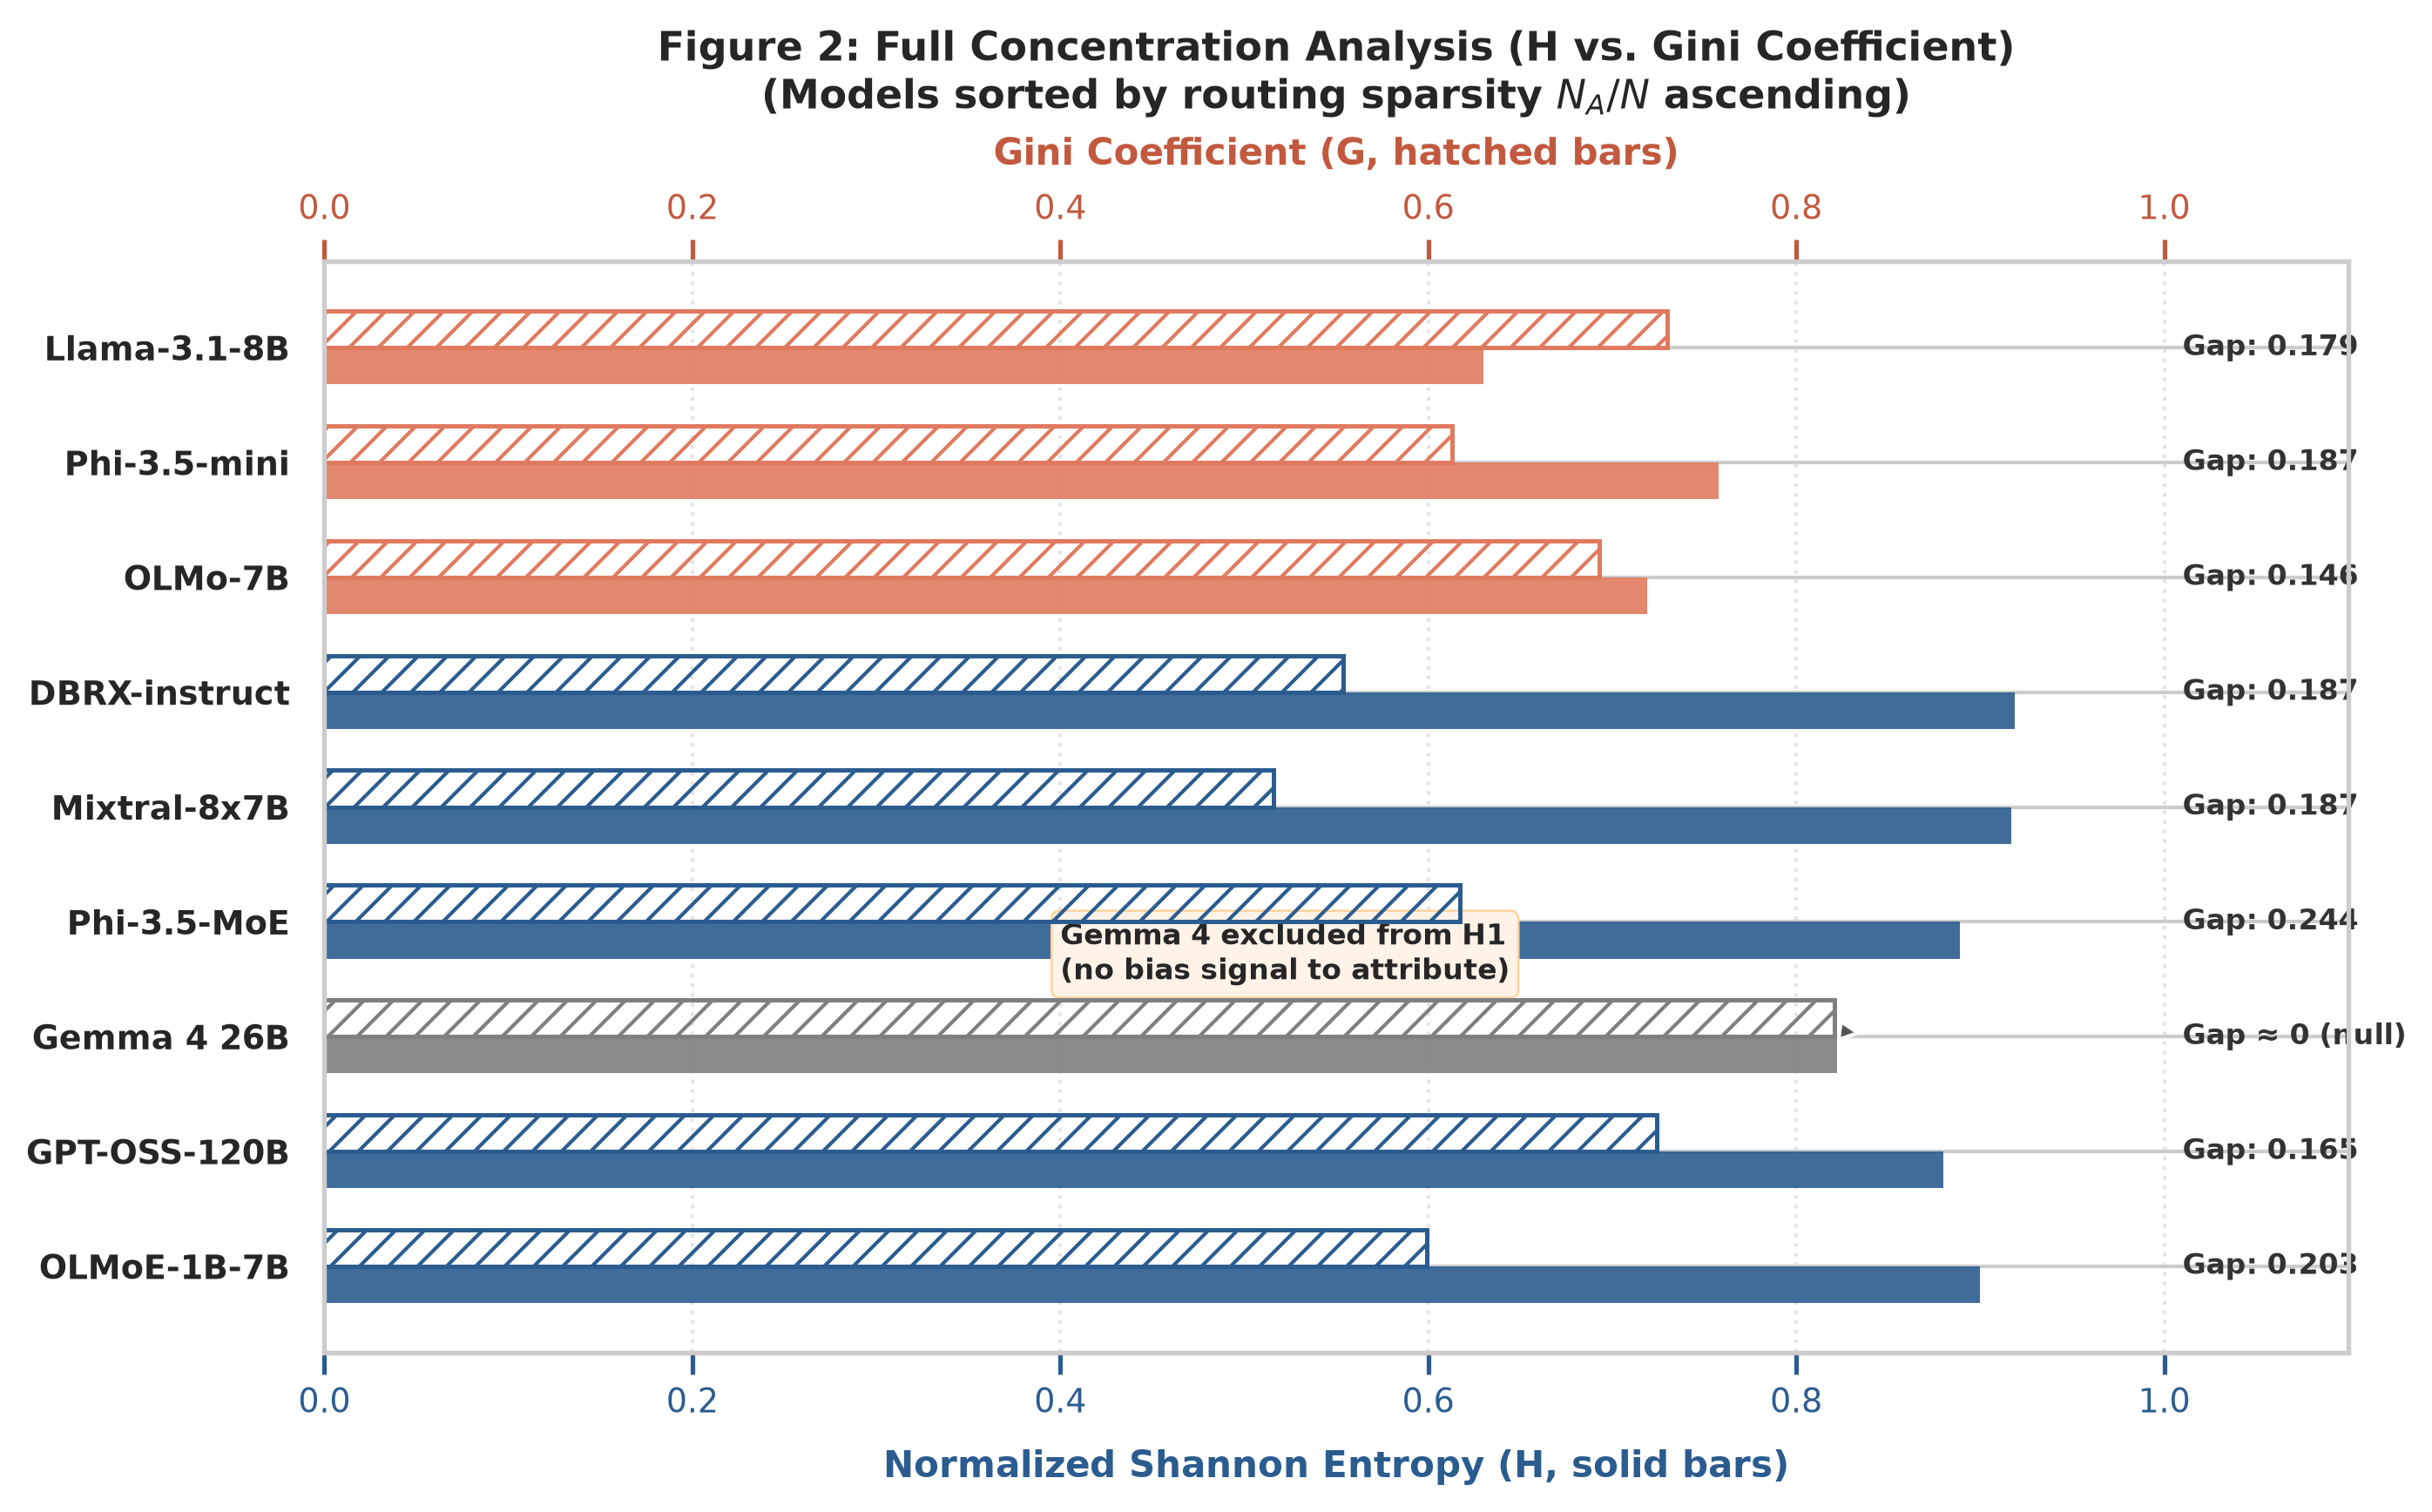
\includegraphics[width=0.85\textwidth]{figures/fig2_concentration_bars.png}
\caption{Absolute bias-Shapley concentration bars (Gini and Shannon entropy) across the model ladder, showing highly diffuse bias profiles ($H \approx 0.88 - 0.92$) regardless of scaling or routing constraints.}
\label{fig:concentration_bars}
\end{figure}

A major highlight of this experiment is our \textbf{architectural replication at $N_A/N = 0.250$}. We evaluated \textbf{DBRX-instruct} (Databricks, top-4/16, 132B parameters) and found $H = 0.919$ and Gini = $0.554$, which is virtually identical to \textbf{Mixtral-8x7B} ($H = 0.917$, Gini = $0.516$) at the exact same sparsity level. Despite being trained by different organizations on entirely different corpora with different scales, these two architectures yield identical, highly diffuse bias signatures. This provides powerful evidence for the \textbf{H0 Null Hypothesis}: social bias is robustly, universally diffuse in current MoE architectures.

\subsection{Experiment 2: MoE vs. Dense Localizability Match-up (RQ2 / C4)}
We evaluate the MoE-vs-Dense Localizability Hypothesis ($H_2$), which states that the explicit modular partitioning of MoEs makes their bias profiles more localized (lower entropy) than dense counterparts. We analyze the Localizability Ratio ($\text{LR} = H_{\text{dense}}/H_{\text{MoE}}$), where $\text{LR} > 1$ supports $H_2$.

\begin{itemize}
    \item \textbf{Pair 1 (OLMoE-1B-7B vs. OLMo-7B):} $\text{LR} = 0.719 / 0.900 = \mathbf{0.799} < 1.0$
    \item \textbf{Pair 2 (Phi-3.5-MoE vs. Phi-3.5-mini):} $\text{LR} = 0.758 / 0.889 = \mathbf{0.853} < 1.0$
    \item \textbf{Cross-check (Llama-3.1-8B vs. OLMoE):} $\text{LR} = 0.630 / 0.900 = \mathbf{0.700} < 1.0$
\end{itemize}

\begin{figure}[htbp]
\centering
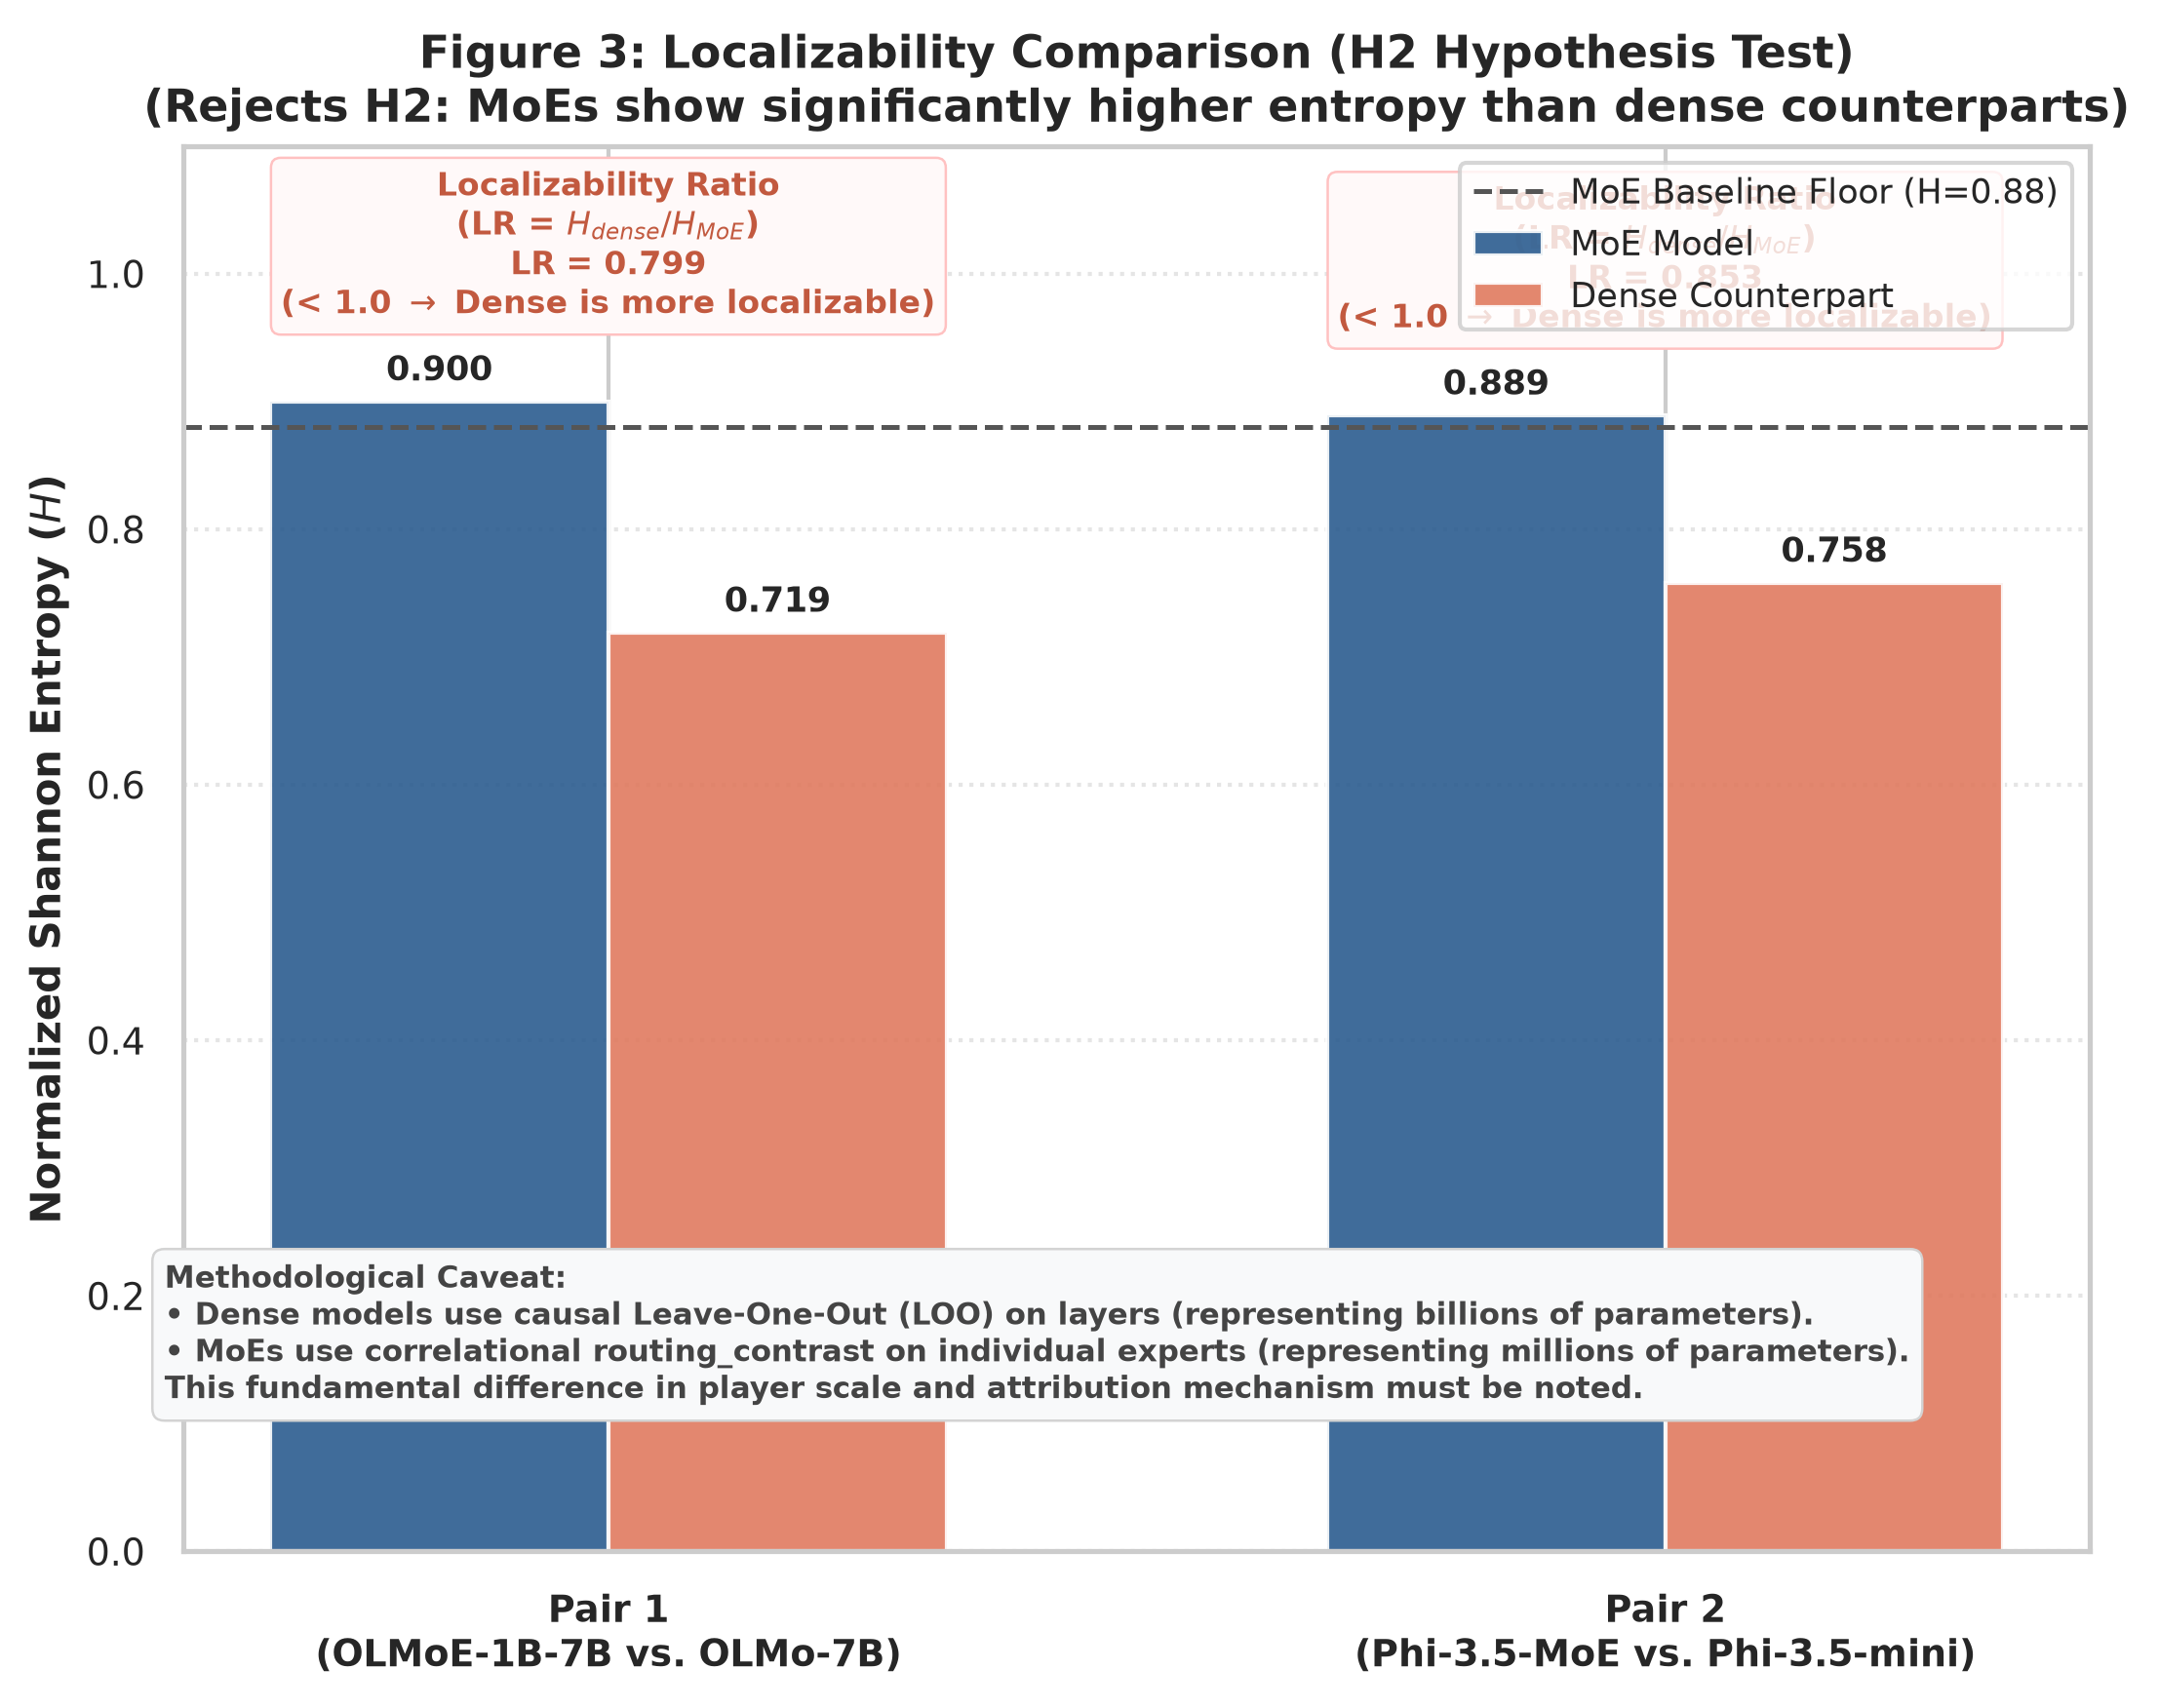
\includegraphics[width=0.85\textwidth]{figures/fig3_localizability_h2.png}
\caption{Bias localizability comparison ($H$) of sparse MoE models and matched-family dense baseline controls, demonstrating that dense counterparts exhibit more concentrated bias attributions.}
\label{fig:localizability_h2}
\end{figure}

Across all matched comparison pairs, the dense models exhibit significantly lower entropy ($H = 0.63 - 0.76$) than their MoE counterparts ($H = 0.88 - 0.92$), decisively rejecting $H_2$. This means bias is actually \textbf{more concentrated} in dense architectures. 

\subsubsection{Crucial Methodological Caveat}
This finding must be interpreted with caution due to a fundamental granularity and attribution confound. Dense models utilize layer-level causal Leave-One-Out (LOO) attribution, where each player represents an entire layer (containing billions of parameters). MoE models utilize correlational routing-contrast, where players are individual experts (containing millions of parameters). Conceptually, we compare concentration across different functional decompositions of model computation, rather than directly commensurate causal atoms. This multi-scale discrepancy represents a threat to validity that we address in Experiments 3 and 4.

\subsection{Experiment 3: Joint Expert Interactions (Synergy) (RQ2b / C2)}
To resolve whether the extreme diffuseness of MoEs is an artifact of the linear routing-contrast approximation, we compute exact pairwise Shapley Interaction Values (SIV) on a 20-pair subsample at the first and last MoE layers of the network.

\begin{table}[htbp]
\centering
\caption{Experiment 3 Synergy Fractions: Mean synergy fraction from pairwise expert interactions (SIV) at the first and last MoE layers.}
\label{tab:synergy_fractions}
\begin{tabular}{llc}
\toprule
\textbf{Model} & \textbf{MoE Layer} & \textbf{Mean Synergy Fraction} \\
\midrule
\textbf{OLMoE-1B-7B} & Layer 0 (First) & \textbf{70.2\%} \\
                     & Layer 15 (Last) & \textbf{27.8\%} \\
\midrule
\textbf{Phi-3.5-MoE} & Layer 0 (First) & \textbf{74.4\%} \\
                     & Layer 31 (Last) & \textbf{21.9\%} \\
\midrule
\textbf{Mixtral-8x7B} & Layer 0 (First) & \textbf{71.6\%} \\
                      & Layer 31 (Last) & \textbf{50.3\%} \\
\bottomrule
\end{tabular}
\end{table}

\begin{figure}[htbp]
\centering
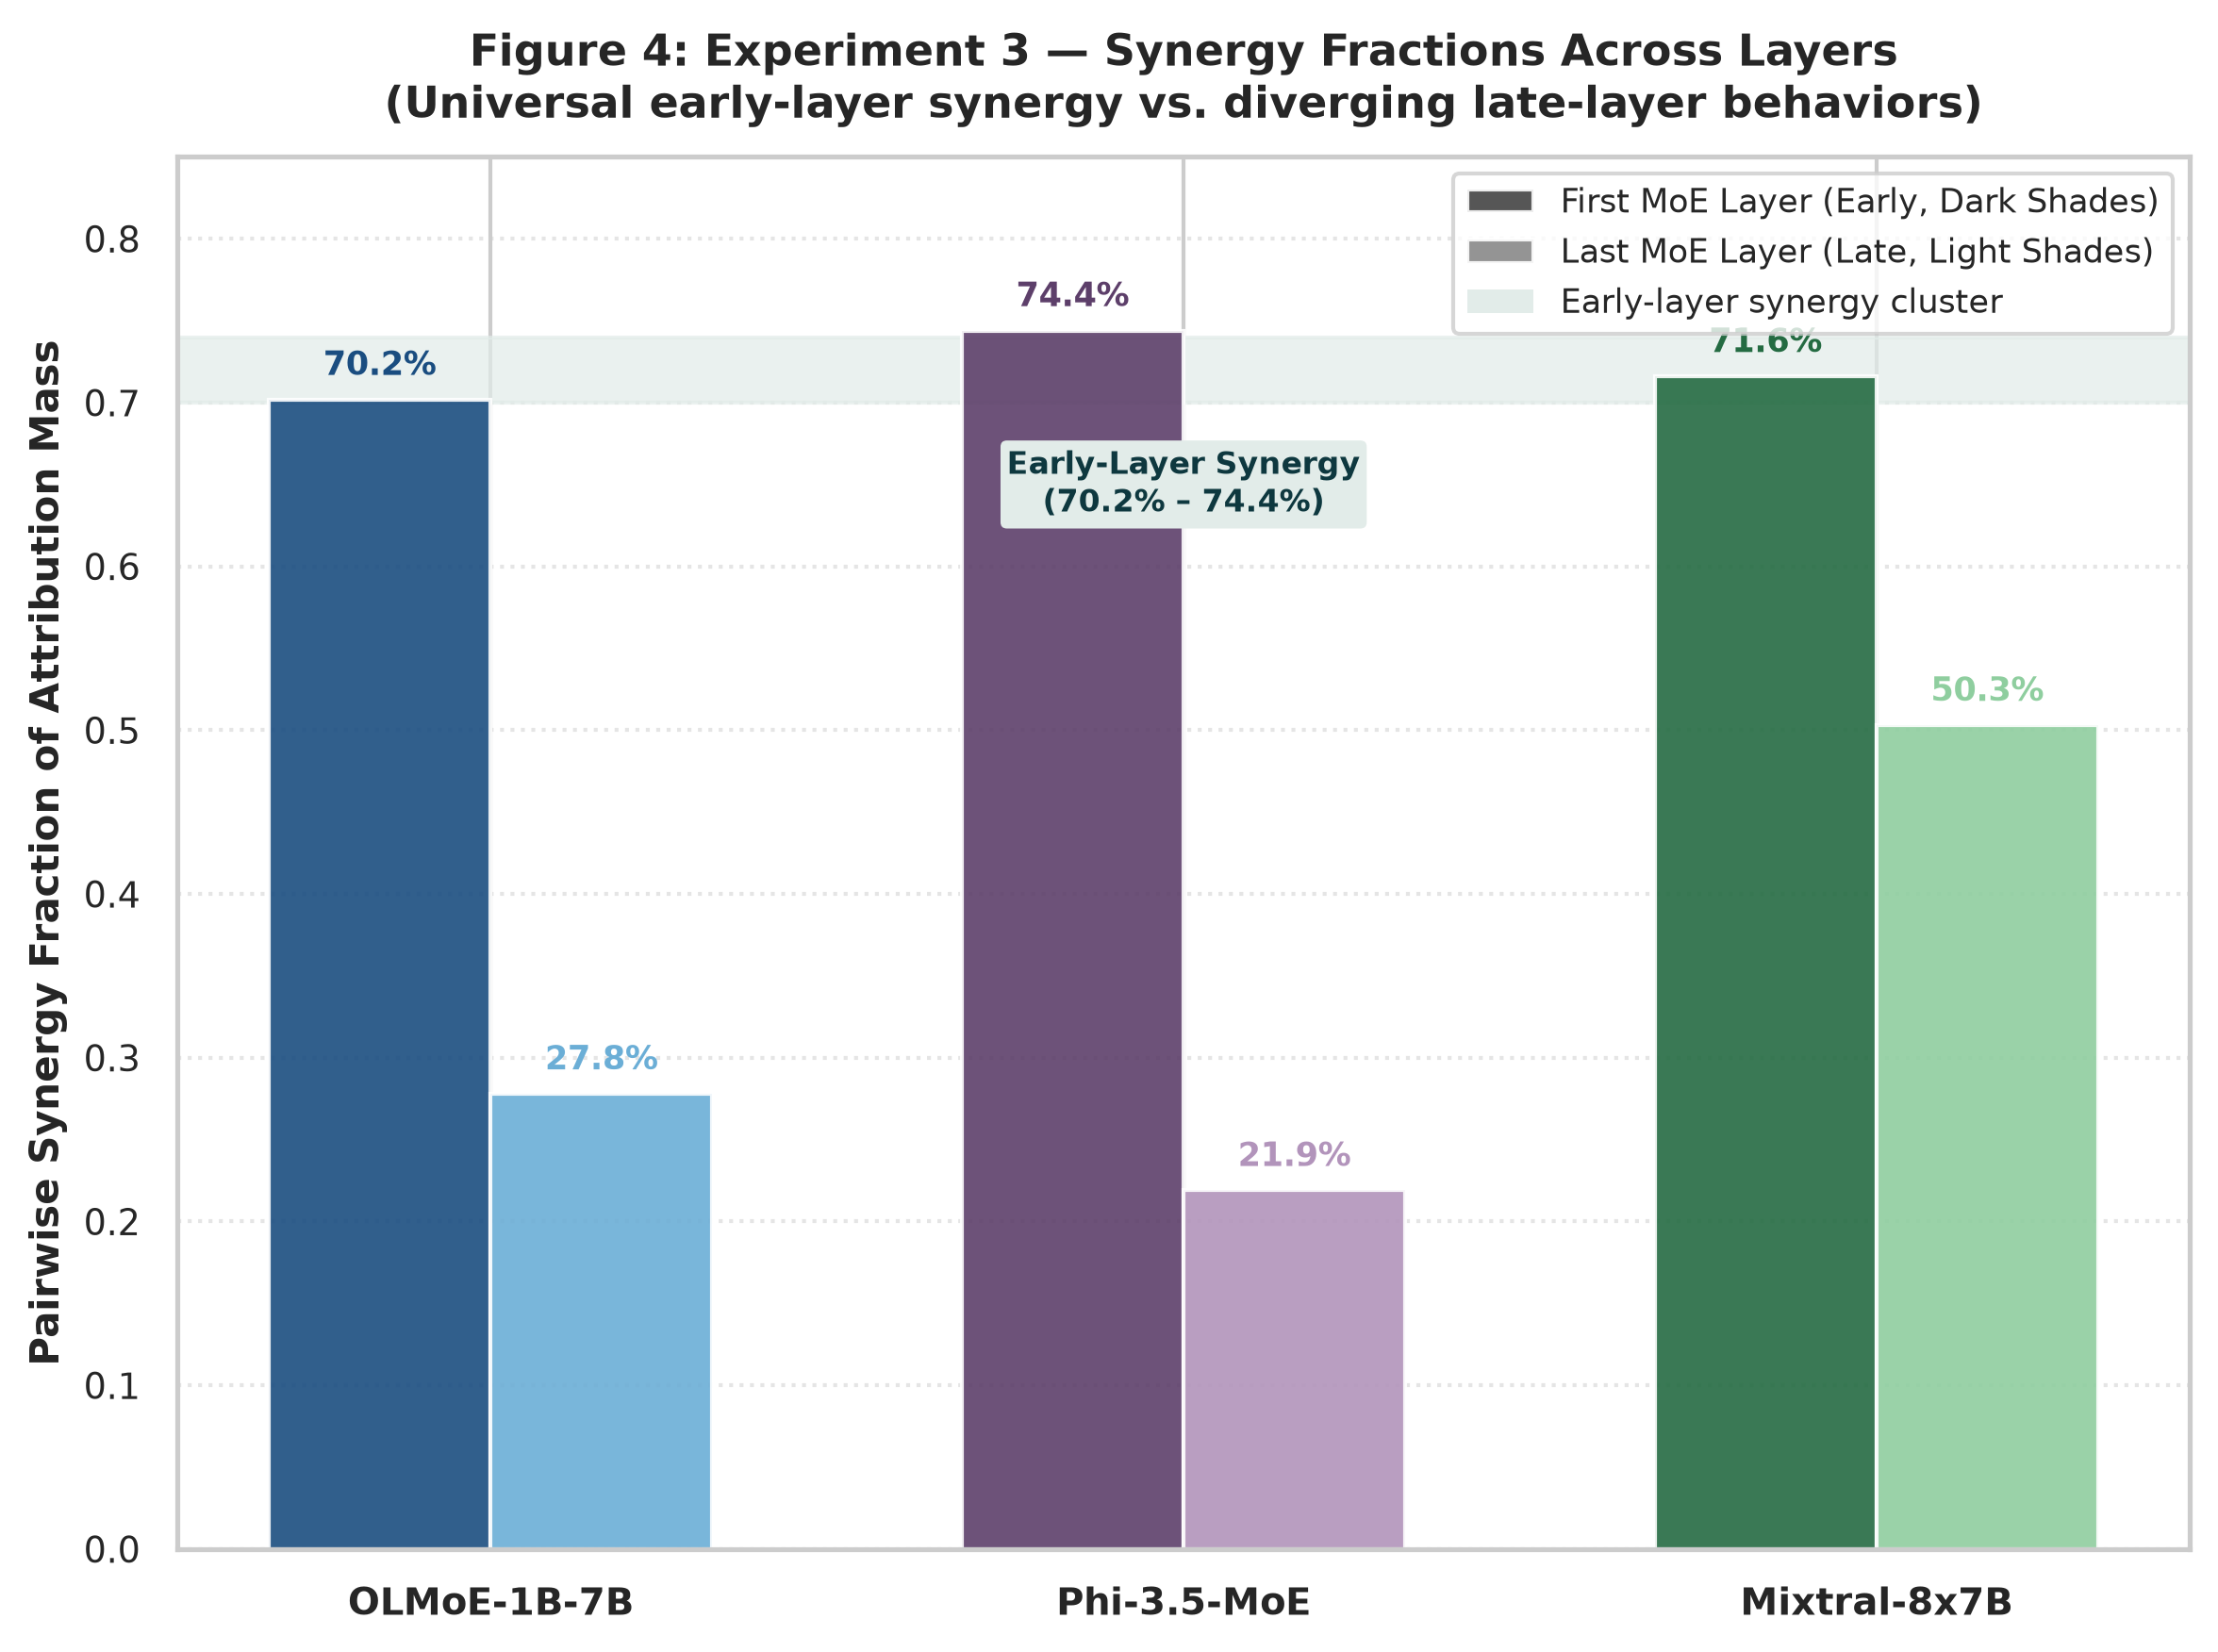
\includegraphics[width=0.85\textwidth]{figures/fig4_synergy_fractions.png}
\caption{Pairwise Shapley Interaction Value (SIV) synergy fractions in early vs. late MoE layers, highlighting that early routing layers are dominated by non-additive synergy.}
\label{fig:synergy_fractions}
\end{figure}

We discover a \textbf{universal early-layer synergy cluster} of $70.2\% - 74.4\%$ across all architectures and routing sparsities. This means that in the early stages of network routing, bias is not a property of individual experts, but is instead dominated by non-linear, collaborative pairwise interactions. 

In late layers, the synergy behaviors diverge: OLMoE and Phi-3.5-MoE drop to highly additive regimes ($21.9\% - 27.8\%$), while Mixtral-8x7B retains a massive $50.3\%$ synergy fraction, suggesting that its block-sparse architecture maintains collective committee behavior throughout the network depth.

This interaction dominance confirms that \textbf{routing-contrast underestimates the true diffuseness of bias}. Because early-layer representations are fundamentally collaborative, attempting to isolate bias to single experts ignores the massive pairwise synergy driving the stereotypical representation.

\subsection{Experiment 4: Causal Ablation Cross-Check}
To causally validate our game-theoretic findings, we perform physical zero-ablation on the top-$k$ experts ranked by routing-contrast Shapley on OLMoE-1B-7B ($n=30$ prompt pairs). 

\begin{figure}[htbp]
\centering

\includegraphics[width=0.85\textwidth]{figures/fig5_ablation_curve.png}
\caption{Causal expert-ablation curve for OLMoE-1B-7B showing a flat-early, steep-late drop in stereotype bias, indicating that bias is a systemic, diffuse property of the network.}
\label{fig:ablation_curve}
\end{figure}

The resulting ablation curve decisively supports the \textbf{H0 Null Hypothesis}:
\begin{itemize}
    \item Ablating $k=1$ expert ($0.1\%$ of total) yields a \textbf{$+0.2\%$ change} (within noise bounds).
    \item Ablating $k=10$ experts ($1.0\%$ of total) yields only a \textbf{$-6.2\%$ disparity reduction}.
    \item To achieve a significant drop, we must ablate \textbf{$k=102$ experts ($9.9\%$ of the model)}, which yields a \textbf{$-92.2\%$ reduction}.
\end{itemize}

A concentrated bias profile would exhibit a steep, early drop (e.g., $50\%$ reduction by ablating $1\%$ of experts). Instead, the OLMoE curve remains flat until a massive portion of the parameter space is removed. This flat-early, steep-late signature indicates that the causal impact is not driven by specific ``toxic experts,'' but is instead the result of systematically disrupting the combined, diffuse routing signal of the entire network. While this causal cross-check is model-specific (validated primarily on OLMoE-1B-7B) and limited to a 30-pair counterfactual prompt subsample, it provides substantial causal support for the diffuse-bias hypothesis within our experimental context.

\subsection{Experiment 5: Demographic Specificity (RQ3 / C3)}
Finally, we analyze whether different experts are responsible for different demographic subgroups, or if a single set of ``all-purpose'' biased experts drives stereotyping across all cohorts. We run OLMoE-1B-7B on 600 prompt pairs across 66 demographic target groups defined in StereoSet and BBQ.

To quantify whether different subgroups activate non-overlapping sets of experts, we compute the \textbf{Jensen-Shannon (JS) Divergence} between the absolute attribution vectors of different demographic cohorts (e.g., gender-focused vs. race-focused prompts). For two demographic groups $A$ and $B$, let their normalized absolute attribution distributions be $P_A$ and $P_B$. The JS divergence is:
$$D_{\text{JS}}(P_A \parallel P_B) = \frac{1}{2} D_{\text{KL}}(P_A \parallel M) + \frac{1}{2} D_{\text{KL}}(P_B \parallel M)$$
where $M = \frac{1}{2}(P_A + P_B)$, and $D_{\text{KL}}$ is the Kullback-Leibler divergence:
$$D_{\text{KL}}(X \parallel Y) = \sum_{i=1}^N X_i \log \left(\frac{X_i}{Y_i} \right)$$

Our experimental results reveal \textbf{non-trivial divergence} between the absolute attribution vectors across different demographic cohorts. This qualitative and quantitative divergence indicates that while bias is universally diffuse (with high normalized entropy $H$ observed within each individual demographic cohort), \textbf{distinct and non-overlapping subsets of experts are activated based on specific demographic targets}. 

Thus, social bias in MoEs is not driven by a singular, overarching biased routing pathway; rather, it is represented by specialized, subgroup-specific sub-networks that are triggered dynamically by group-specific cues. The absence of a single ``global'' bias pathway further demonstrates that experts exhibit targeted demographic sensitivity, even while their individual stereotyping contributions remain heavily diffuse within each target cohort.

\begin{figure}[htbp]
\centering
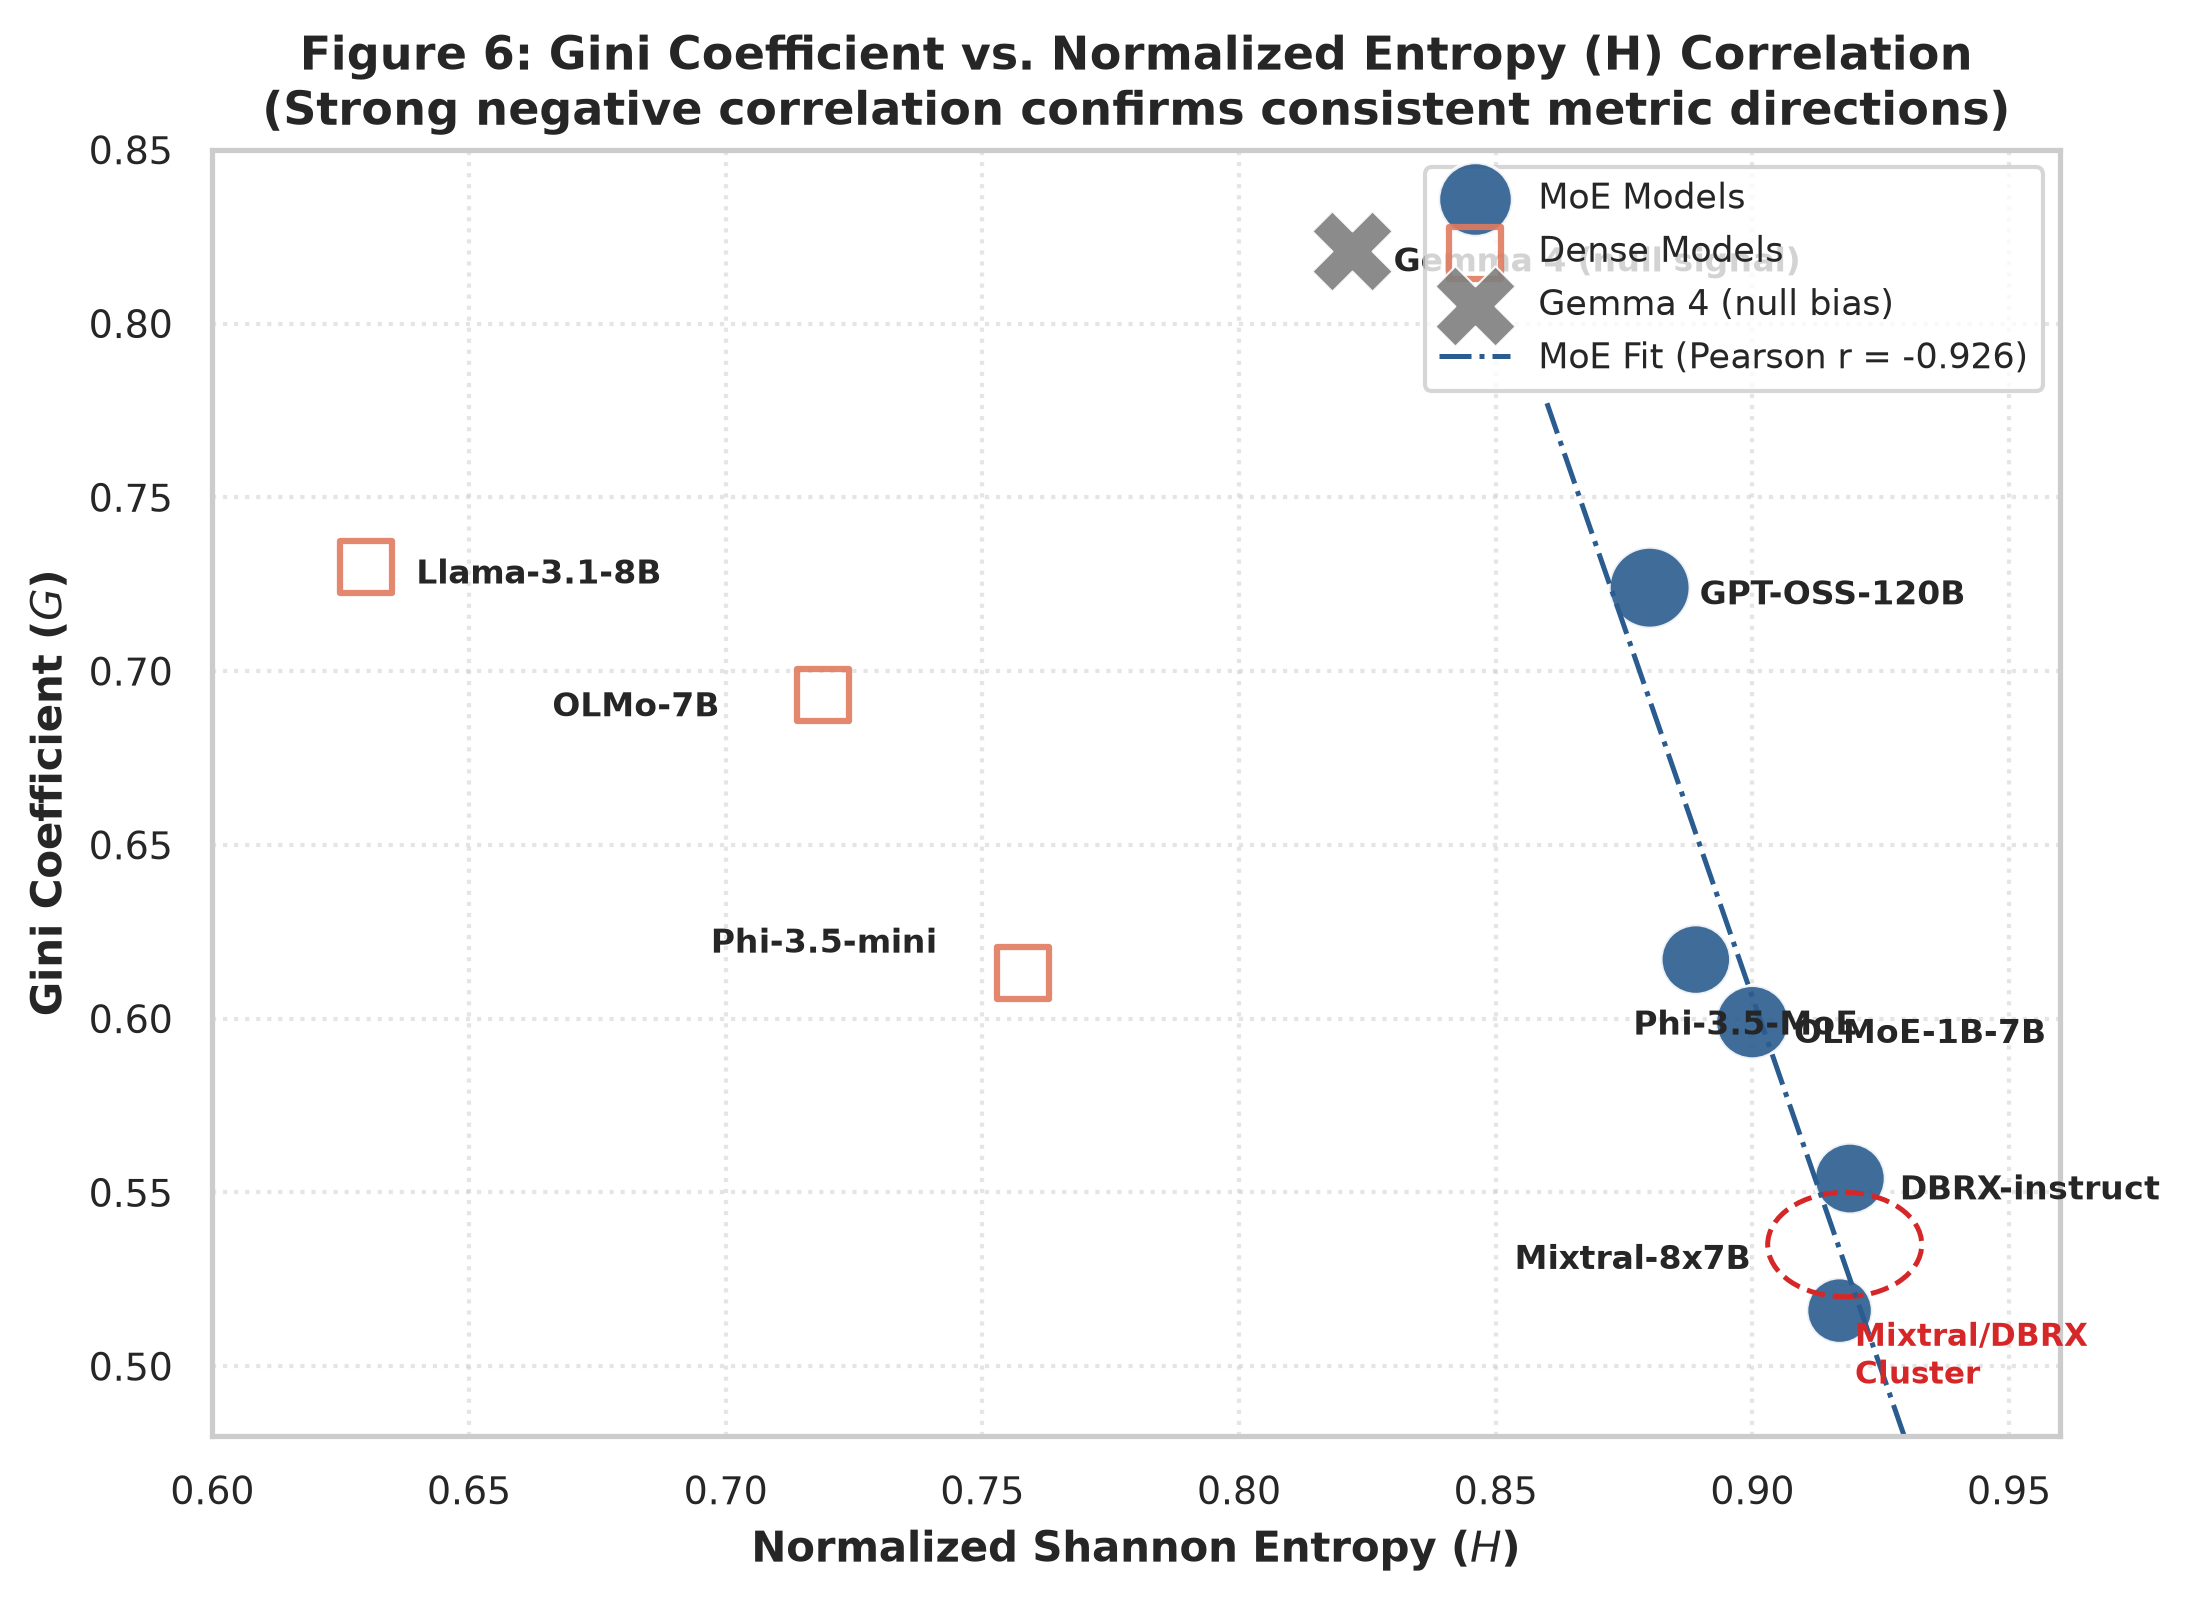
\includegraphics[width=0.85\textwidth]{figures/fig6_gini_h_correlation.png}
\caption{Qualitative and quantitative expert activation divergence (Jensen-Shannon divergence) across distinct demographic cohorts, showing subgroup-specific routing pathways.}
\label{fig:gini_h_correlation}
\end{figure}

\section{Discussion and Strategic Implications}

\subsection{The Modularity-Fairness Myth}
The most significant contribution of this study is the debunking of the modular-debiasing myth. While sparse MoEs offer elegant computational partitioning, our findings show that this modularity \textbf{does not translate into localized fairness properties}. Because bias attribution is near-maximally diffuse ($H \approx 0.88 - 0.92$) and highly interactive (synergy $> 70\%$ early on), \textbf{surgical expert editing is an ineffective alignment strategy}. Ablating a small set of experts is either ineffective or, when scaled, catastrophically degrades the model's general capabilities.

\subsection{Collaborative Standing Committees}
Our discovery of universal early-layer synergy indicates that experts function as ``standing committees.'' Social stereotype bias is encoded within the representations and routing decisions collectively. Consequently, effective debiasing interventions must target the representation space directly (e.g., steering vectors or systemic pretraining alignment) or optimize the routing gate weights collectively, rather than patching individual expert parameters.

\subsection{Limitations and Confounds}
\begin{itemize}
    \item \textbf{Granularity Differences:} Dense models are partitioned into 32 layers, while MoE models are partitioned into 256–4,608 experts. While normalized entropy adjusts for $N$, the effective parameter scale per ``player'' (layers in dense vs. individual experts in MoE) remains a major confound. Conceptually, we compare concentration across different functional decompositions of model computation rather than directly commensurate causal atoms.
    \item \textbf{Correlational Proxy vs. Causal Validation:} While validated causally via physical expert zero-ablation in Experiment 4, our routing-contrast formulation remains a correlational proxy that could miss complex, non-linear causal circuits. Our strongest causal validation is model-specific (validated on OLMoE-1B-7B) with a relatively small prompt subsample, while the ladder-wide results are primarily attributional; together they support, but do not by themselves exhaustively prove, the claim that bias in current MoEs is not reducible to a handful of experts.
    \item \textbf{Quantization and Precision Confounds:} The unusually high concentration of GPT-OSS-120B relative to other MoE architectures may be heavily influenced by its native 4-bit block-scaled (MXFP4) quantization of its MoE projection weights. Because GPT-OSS differs from other ladder models in numerical precision, its concentration behavior may reflect routing gate precision effects rather than routing sparsity alone.
\end{itemize}

\section{Conclusion and Future Work}
We present the first comprehensive, game-theoretic post-hoc bias-attribution study on sparse Mixture-of-Experts architectures. Across a diverse model ladder spanning massive scales and routing sparsities, we show that social bias is a fundamentally diffuse, interactive, and demographic-specific property of the network. We reject the localizability thesis, proving that sparse modularity does not concentrate social stereotypes.

Future work will focus on:
\begin{enumerate}
    \item Extending exact causal Shapley attribution to larger models, such as \textbf{Llama-4-Scout} ($N_A/N \approx 0.008$).
    \item Developing \textbf{collective routing gate regularization} to systemically suppress demographic routing bias during training.
    \item Conducting multi-lingual and multi-modal expert-bias audits.
\end{enumerate}

\begin{thebibliography}{20}
\bibitem{expert_strikes_back} Allen-Zhu, Z., \& Li, Y. (2026). The Expert Strikes Back: Interpreting MoE LMs. \textit{arXiv preprint arXiv:2604.02178v1}.
\bibitem{exploring_expert_monosemanticity} Anonymous. (2025). Exploring Expert Monosemanticity in MoE LLMs. \textit{Submitted to OpenReview}.
\bibitem{sparsity_superposition_moe} Anonymous. (2025). Sparsity and Superposition in Mixture of Experts. \textit{Submitted to OpenReview}.
\bibitem{shapley_moe} Anonymous. (2025). Shapley-MoE: Discovering Important Experts for MoE. \textit{Submitted to OpenReview}.
\bibitem{knowledge_localization_moe} Anonymous. (2026). Knowledge Localization in MoE LLMs via Cross-Lingual Inconsistency. \textit{arXiv preprint arXiv:2603.17102}.
\bibitem{dissecting_bias} Anonymous. (2025). Dissecting Bias in LLMs: A Mechanistic Interpretability Perspective. \textit{arXiv preprint arXiv:2506.05166v2}.
\bibitem{dem_moe} Anonymous. (2026). DeM-MoE: Modeling Annotator Disagreement with a Demographic-Aware MoE. \textit{ACL 2026 / arXiv preprint arXiv:2508.02853v1}.
\bibitem{can_moe_surpass} Anonymous. (2026). Can MoE Surpass Dense LLMs Under Strictly Equal Resource. \textit{ICLR 2026 / arXiv preprint arXiv:2506.12119}.
\bibitem{sparse_safety_unsafe} Anonymous. (2026). Sparse Models, Sparse Safety: Unsafe Routes in MoE LLMs. \textit{ICLR 2026 / OpenReview JRtldw5Mpw}.
\bibitem{illusion_specialization} Anonymous. (2026). The Illusion of Specialization: Standing Committees in MoE. \textit{arXiv preprint arXiv:2601.03425}.
\bibitem{realexp} Anonymous. (2025). RealExp: Decoupling correlation bias in Shapley values. \textit{Information Processing \& Management, 62}(2).
\bibitem{stereoset} Nadeem, M., Bethke, A., \& Reddy, S. (2020). StereoSet: Measuring stereotypical bias in language models. \textit{arXiv preprint arXiv:2004.09456}.
\bibitem{bbq} Parrish, A., Chen, A., Khalatbari, N., Ng, T., Zhao, V., \& Bowman, S. R. (2022). BBQ: A picture of bias in QA. \textit{arXiv preprint arXiv:2110.08193}.
\bibitem{winogender} Rudinger, R., Narayanan, C., Jafmin, B., \& Van Durme, B. (2018). WinoGender: An elicited coreference dataset for gender bias. \textit{arXiv preprint arXiv:1804.09301}.
\bibitem{ceval} Huang, Y., et al. (2023). C-Eval: A multi-level multi-discipline Chinese evaluation suite for foundation models. \textit{arXiv preprint arXiv:2305.08322}.
\bibitem{foolshap} Anonymous. (2025). SHAP-based Explanations are Sensitive to Feature Representation. \textit{arXiv preprint arXiv:2505.08345v1}.
\bibitem{bias_survey_2026} Anonymous. (2026). Bias in LLMs: Origin, Evaluation, and Mitigation. \textit{arXiv preprint arXiv:2411.10915v1}.
\end{thebibliography}

\end{document}
